\section{Motivation}\label{sec:motivation}
Efficient team schedule planning is a complex challenge, particularly in organizations that require real-time coordination and resource management.
Existing scheduling services often have significant limitations, such as proprietary nature, lack of customization, and dependence on third-party infrastructure.
This highlights the need for tailored solutions that can address specific organizational requirements more effectively.
This project aims to develop a self-hosted open-source booking system designed for organizations that need a private, adaptable scheduling solution.
The system will provide a web-based interface where users can:
\begin{itemize}
    \item Make and manage reservations
    \item Check real-time room availability
    \item  Filter bookings by person or room
    \item View all reservations on a centralized calendar
\end{itemize}

The backend will be built using the Spring Framework, ensuring scalability, security, and ease of integration with existing infrastructure.
Unlike cloud-based alternatives, this system will store all data locally, giving organizations complete privacy and control over scheduling information.
By combining flexibility, transparency, and data privacy, this project can provide a practical alternative to commercial scheduling tools, empowering organizations with greater autonomy and customization options.

\newpage

\section{The current solution}\label{sec:the-current-solution}
\begin{figure}[h]
    \centering
    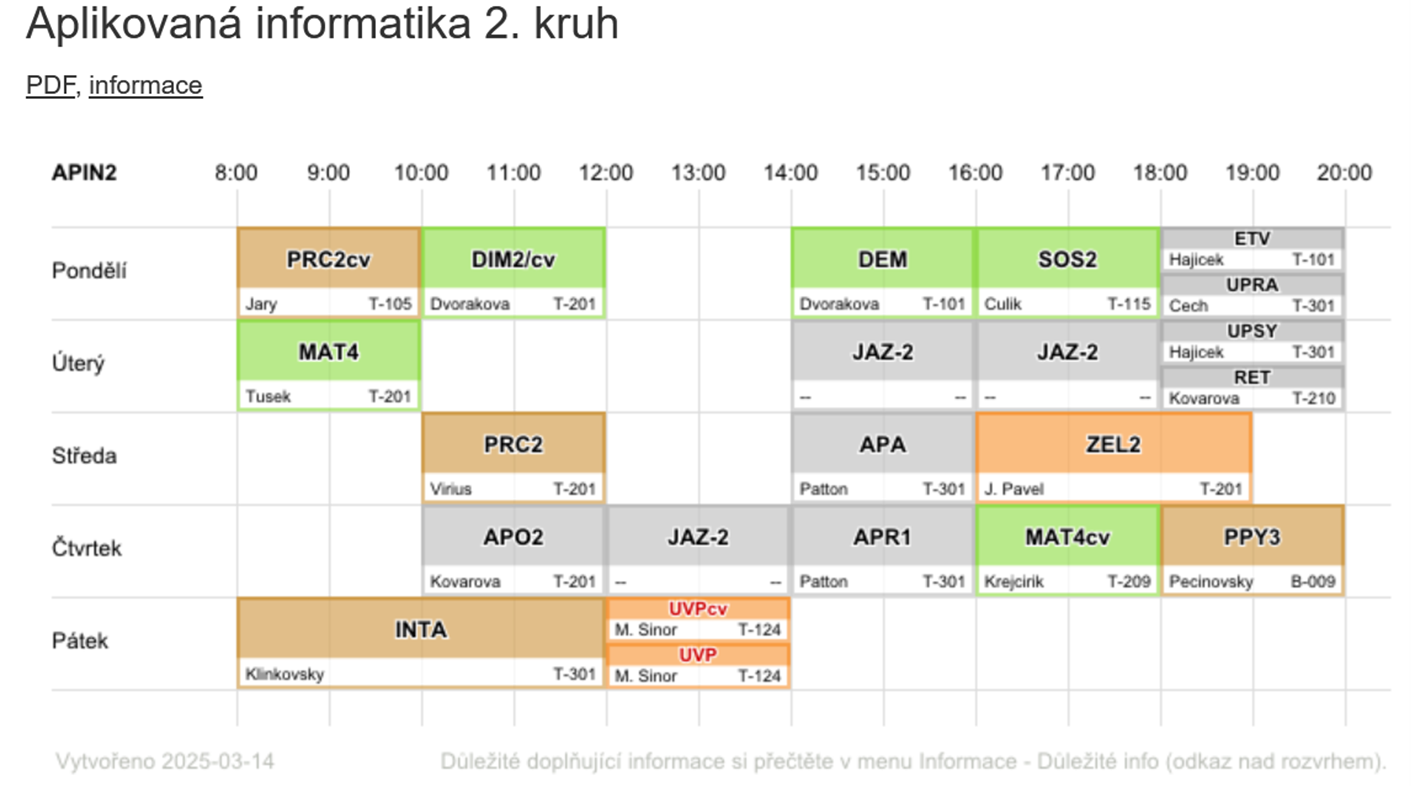
\includegraphics[width=0.6\textwidth]{img}
    \caption{Screenshot of the current solution}
    \label{fig:rozvrh}
\end{figure}
Initially, it is needed to examine the existing solution employed by my institution, CTU. The website Rozvrh.fjfi.cvut.cz serves as a platform where students can view their academic schedules.

It can be seen in fig.~\ref{fig:rozvrh} that while the website completes its main purpose, it is not customizable, making it difficult to use.
The current implementation presents several significant limitations that impact the user experience and efficiency.

\textbf{Limited Customization}: The system lacks personalization features, forcing all users to view the same static schedule format regardless of their specific needs or preferences.

\textbf{Cross-Program Scheduling Complexity}: Students enrolled in classes over different years or programs face particular challenges.
They must manually navigate between multiple schedule views and compare information from different sources.
This process is not only time-consuming, but is also prone to errors.

\textbf{Manual Workarounds}: The limitations of the current system have led to widespread adoption of inefficient workarounds.
Many students resort to taking screenshots of their schedules and manually marking or crossing out irrelevant classes.
This practice, while common, introduces several problems:
Increased risk of scheduling conflicts due to manual tracking,
difficulty in keeping track of schedule updates,
time wasted on manual schedule management,
potential for missed classes due to human error.


These limitations highlight the urgent need for a more sophisticated scheduling solution.
A modern calendar system should address these issues by providing:

\textbf{Personalization}: Allow users to customize their view based on their specific needs and preferences.

\textbf{Cross-Program Integration}: Enable seamless viewing of classes across different programs and years.

\textbf{Digital-First Approach}: Eliminate the need for manual workarounds by providing a comprehensive digital solution

This project aims to develop such a solution, focusing on creating a calendar system that is not only functional, but also user-friendly and customizable.


\section{Thesis Aims and Objectives}\label{sec:thesis-aims}
The primary objective of this thesis is to explore and evaluate Java-based web development libraries while designing and implementing a practical team-work organization application.
This project aims to demonstrate the application of modern Java web technologies in creating a functional and user-friendly system for team collaboration.

\subsection{Primary Objectives}\label{subsec:primary-objectives}
The development process is guided by several key objectives that form the foundation of this project.
These objectives are designed to ensure a systematic and comprehensive approach to the development of the team-work organization system.

The first step focuses on the \textit{exploration and evaluation of technology}.
In this phase, we will conduct comprehensive research into available Java web development libraries and frameworks.
This exploration will encompass various aspects including web application development, database integration, user interface implementation, and security measures.
Based on this research, we will carefully select and document the most appropriate technologies for the project's specific requirements.

The second objective involves a thorough \textit{requirement analysis}.
This phase will identify and document all the functional requirements necessary for effective team-work organization.
Additionally, we will establish non-functional requirements covering performance expectations, security needs, usability standards, scalability considerations, and maintainability requirements.
This comprehensive analysis will ensure that the system can meet both immediate and long-term organizational needs.

\textit{The system design} is the third stage, where we will develop a complete system architecture incorporating the selected technologies.
This includes designing an efficient database schema for the team work organization, creating detailed user interface mockups, defining system components and their interactions, and establishing a robust security architecture.
The design phase will focus on creating a scalable and maintainable system structure.

\textit{Implementation} forms the fourth phase, where we will develop core functionalities essential for the system's operation.
This includes comprehensive user management capabilities, room creation and management features, event assignment and tracking systems, and advanced event displaying and filtering options.
The implementation will also incorporate robust security measures, a responsive user interface, and ensure complete data integrity throughout the system.

The final stage focuses on \textit{testing and validation}.
This phase will involve developing and executing comprehensive test cases at multiple levels, including unit testing, integration testing, and user acceptance testing.
We will verify all system functionality against the established requirements, document test results and any issues discovered, and implement necessary improvements based on testing outcomes.
This thorough testing approach will ensure the reliability and effectiveness of the system in real-world applications.
\newpage

\subsection{Expected Outcomes}\label{subsec:expected-outcomes}
The successful completion of these objectives will result in:

\begin{itemize}
    \item \textbf{A comprehensive understanding} of Java web development libraries and their practical applications

    \item \textbf{A functional application} for team work organization that:
    Facilitates efficient team collaboration,
    Provides intuitive event management,
    Ensures secure interactions with the system,
    Offers responsive and user-friendly interface.


    \item \textbf{Detailed documentation} covering: technology evaluation and selection process,
    system architecture and design decisions,
    implementation details, testing methodology, and results.


    \item \textbf{Practical experience} in: Java web application development,
    database design and implementation,
    user interface development,
    system testing and validation.
\end{itemize}
